
\section{Introduction}

With increasing diversity, there have been renewed debates concerning the performance of diverse teams when it comes to creativity and problem-solving. If diverse teams outperform homogeneous teams, this would offer an additional argument for broader inclusion, and hold clear practical lessons for decision-makers. Some of the foundational research in this field has been computational, yet replications are lacking. This paper offers a direct replication of the most influential model in the field, presented by Hong and Page in 2004\supercite{hong_groups_2004}, and a replication of a recent paper by Grim et al.\supercite{grim_diversity_2019} that offered important qualifications. By doing so with the use of an agent-based modeling framework that easily allows for extensions and adjustments to the model, this replication will also be helpful for future research into the conditions under which diversity may trump ability. \\

Seventeen years ago, Hong and Page\supercite{hong_groups_2004} proposed that diversity generally trumps ability when it comes to the composition of groups of problem solvers. To support this argument, their paper, which has been cited more than 1,400 times, presented the results of an agent-based model. While similar models have been used in further research \supercite{singer2019diversity, grim_diversity_2019, holman2018diversity}, no direct replication has been published, and neither the original paper nor any of the derivations provide open code. Recent research has proposed qualifications to the original conclusions, and by replicating one of the most critical recent papers\supercite{grim_diversity_2019}, I show that these concerns deserve further and more nuanced consideration.  

\subsubsection{The basic model}

To explore the process of problem-solving, Hong and Page tasked teams of agents with finding the highest value in a ring of 2,000 random numbers. These values can be thought of as representing the quality of 2,000 possible solutions to a problem that the agents want to solve, such as maximizing the time users spend on an online platform. Each agent approaches this task with a distinct heuristic that consists of an ordered set of non-repeating integers $\{h_{1}, h_{2}, h_{3}\}$. From their current position on the ring, they look forward $h_{1}$ steps and move to that position if its value is greater than that of the current position. Otherwise, they stay put. They then try $h_{2}$ steps, $h_{3}$, $h_{1}$ steps again, and so on, until none of the three checks yields a higher value and thus a move. When they are in a team, the agents take turns. The active agent moves as far ahead as their heuristic allows them to, and then summons their entire team to that position. The next agent searches from that position, and again the entire team moves to the maximum value that this agent can reach (if that agent can achieve any improvement). This process is repeated until none of the agents can move their team any further.

To explore the trade-off between individual agents' abilities and a group's diversity, Hong and Page needed to define these constructs. Given that each agent's heuristic results in a unique end point from any given starting point, their \emph{ability} was defined as the average value of the end points reached from every possible starting point. A group's \emph{diversity} was defined as the average percentage with which any pairs of heuristics do not overlap. For example, $\{1, 2, 3\}$ and $\{1, 3, 5\}$ only overlap in one place, while $\{3, 4, 5\}$ and $\{4, 5, 6\}$ do not overlap at all.\footnote{Note that Singer\supercite{singer2019diversity} showed that a different measure of diversity - \emph{coverage diversity}, i.e. the share of possible steps covered by at least a single member of the group - more directly predicts a group's performance.} The key result of the initial study was that groups of the highest-ability agents are less diverse than randomly selected groups, and thus identify worse solutions.

\subsubsection{Grim and colleagues' extension and qualification}

In a random landscape, such as that used by Hong and Page, there are no heuristics that consistently outperform others. Instead, agents' ability is unrelated between one problem landscape and the next. Grim and colleagues pointed out that this is a rather peculiar situation, as problem-solving in most domains benefits from expertise, i.e. from the use of heuristics that tend to be successful across problems. In their model, they vary the randomness of the landscapes by specifying the average distance between points that are randomly assigned and then establishing smooth gradients between them. In settings with lower randomness, problems (i.e. landscapes) are more similar to each other, so that the correlation between a heuristic's performance on different problems increases. In such settings, they find that teams selected based on their ability outperform randomly selected (and thus more diverse) teams by finding better solutions (i.e. higher peaks) in the landscapes. They also find that the strategy employed by the teams matters; this will be discussed with the results below.

\section{Approach}

The model formulation used in this paper is the same as that used in the original paper by Hong and Page, with the addition of the smoothing parameter and the choice of strategy in the replication of the findings by Grim and colleagues.

\subsubsection{Implementation}

To replicate the two papers, and support future research, I implemented the model in Python, using the mesa framework\supercite{kazil2020utilizing}. This yields readable explicit code, and the derivation of the 'Grim-model' from the 'Hong and Page' model might serve as an example for future model adaptations. While Hong and Page (2004) reported results based on 50 random landscapes and Grim and colleagues relied on 100 runs, the key replications here are based on 500 landscapes. Broader parameter sweeps that establish boundary conditions for the results reported by Grim et al. are based on 100 landscapes for each setting. In the supplementary material, instructions for deploying these scripts to Google Cloud Engine are provided, which allows to reproduce all numerical results in just over 24 hours on 32 cores.

\subsubsection{Parameters}

Problems are characterized by the number of possible solutions, i.e. values on the circle (\emph{N}). In line with the papers to be replicated, this is set to 2000. Heuristics are defined by the number of positions considered by each agent (\emph{k}), which is set to three steps, and the range of step sizes to be considered (\emph{l}). Here, parameter values of 12 and 20 are considered to replicate Hong and Page, while a full sweep from 4 to 30 is conducted to assess the robustness of the results presented by Grim and colleagues. Finally, groups of agents are characterized by their size, which is set to be either 10 or 20 agents for Hong and Page, and 10 agents for Grim and colleagues\footnote{Note that Grim and colleagues used teams of 9 agents. Here, I consistently used 10 agents to ensure that divergences from Hong and Page are not explained by this difference.}.

\subsubsection{Focus}

To enable direct comparisons between the replication results and the original papers, I focus on replicating Table 1 in Hong and Page's paper, and Figures 2, 6 and 9 in Grim and colleagues' paper, since they provide the foundation for their main conclusions. Where discrepancies arise, I present further analyses to explore their causes.

\section{Results}

\subsection{The basic model: Hong and Page}

\begin{table}[htbp]
    \centering
    \begin{tabular}{lllll}
      \toprule
      N & l & Team type &        Solution       & Diversity\\
      \midrule
      10 & 12 & highest-ability &  92.34 (1.26) &  84.63 (4.24) \\
         &    & random &  94.35 (0.56) &  91.75 (2.52) \\
         & 20 & highest-ability &  93.55 (1.25) &  87.06 (4.54) \\
         &    & random &  95.73 (0.48) &  95.06 (1.77) \\
      \midrule
      20 & 12 & highest-ability &  93.66 (0.82) &  85.79 (3.01) \\
         &    & random &  94.74 (0.47) &  91.82 (1.12) \\
         & 20 & highest-ability &   95.0 (0.83) &  88.52 (3.36) \\
         &    & random &  96.48 (0.42) &  95.05 (0.91) \\
      \bottomrule
      \end{tabular}
    \caption{\label{tab:HP}Results of 500 runs of Hong \& Page model, with SD in parentheses}
    \end{table}

    
The replication confirmed the pattern of results observed by Hong and Page, as can be seen in Table \ref{tab:HP}. Random groups of agents outperformed groups of only the high-ability agents in each of the four scenarios, and the observed performances were generally similar here and in the target paper. However, there are two notable divergences. Firstly, the \textit{standard deviations} reported by Hong and Page and those observed here vary by orders of magnitude. For instance, the standard deviation of the performance of groups of 10 highest-ability agents with \textit{l} = 12 observed here was 1.26 while Hong and Page report 0.020. However, this is simply due to the fact that Hong and Page's standard deviations are those of the means, i.e. what are more commonly called standard errors, while I present standard deviations of the observed variables.\footnote{Scott Page clarified that their table showed standard errors in personal communication. Standard errors are standard deviations divided by the square root of the sample size. Where Hong \& Page report the standard error of the diversity of random agents as 0.232, this can thus be converted to a standard deviation by multiplying with the square root of 50, resulting in 1.64. Given the small sample size, this does not differ substantially from the standard deviation of 2.52 observed in my simulations. Their standard errors for the solutions are based on 100,000 runs (50 runs starting from 2000 locations), so that their standard error of 0.007 for random teams indicates a standard deviation of 0.7, again fairly close to my result of 0.56. I am not presenting standard errors here, given that they are a function of the number of runs and would thus not be comparable when running a number of replications in line with what can be expected with current computing resources. Standard deviations, on the other hand, can give a useful indication of the distribution of results around the means reported. Additionally, the fact that the runs to obtain performance figures are not independent but clustered within landscapes suggests that the calculation method used by Hong \& Page might not give a reliable indication of precision for the performance measures in any case. Clustered standard errors seem to be needed for that.} \\

Less straight-forwardly, the \textit{observed diversity in the high-ability teams} diverges substantially. In my replications, it was 85 to 88\%, compared to 71 to 75\% reported in Hong and Page. Given that the observed diversity within random groups is very close to that reported by Hong and Page, it appears unlikely that the discrepancy is due to differences in the calculation of diversity. In another replication of the model, Singer \supercite{singer2019diversity} reports very similar diversity scores to those obtained here (i.e. 87.9 \% for groups of 10 with l = 20). In an email exchange with Scott Page and Daniel J. Singer, we concluded that this suggests that there appears to be a mistake in the calculation of diversity scores for the high-ability teams in the original paper. \\

Regarding the size of the effect, one might wish to note that the results obtained by 10 randomly selected agents with heuristics including step-sizes of up to 12 were only exceeded by groups of 20 highest-ability agents using more expensive heuristics, with step sizes ranging up to 20. 
    
\subsection{Expansion to smoothed landscapes: Grim et al.}

\begin{figure}
    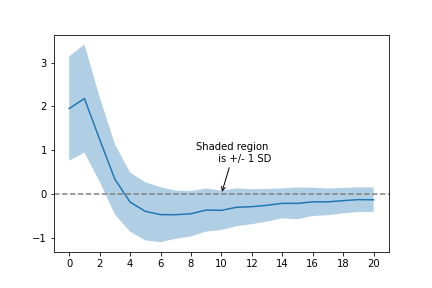
\includegraphics[width=\linewidth]{Fig2.png}
    \caption{Average performance of random minus high-ability teams over 500 random landscapes}
    \label{fig:Grim2}
  \end{figure}
 
 Grim and colleagues extended the model to test whether the degree of smoothness across the solution landscape makes a difference. For fully random landscapes, their paper and my replication thereof, confirms the analysis by Hong and Page: randomly selected teams outperform teams of the highest-ability agents by some 2\%-age points. However, once the landscapes are smoothed, the advantage is reduced. In fact, above a smoothness (i.e. average distance between randomly set points) of 4, 'ability trumps diversity.' My replication results in Figure \ref{fig:Grim2} closely match those presented by Grim et al. in their Figure 2.\footnote{Note that Grim and colleagues report performance in this section of their paper with values below 1. This does not match their claim that they "average the values of the final heights reached when starting from each of 2,000 points [in a range from 1 to 100]" (p. 107), but it seems very likely that this is just a slip from percentages to fractions. For consistency, I report all performance scores here within the range of 1 to 100.} However, the addition of standard deviations to the figure highlights an important point that might go unnoticed in the original presentation: while ability trumps diversity on average on the smoother landscapes, this effect is much smaller than the reverse observed on more random landscapes and also less consistent. Also, it should be noted that the performance of both types of teams declines drastically with increasing smoothness, from 92-94\% on fully random landscapes to less than 70\% on landscapes with a smoothness factor greater than 12.
 
 \subsubsection{Tournament dynamics and further comparisons}
 
 Apart from proposing that ability trumps diversity on smoother landscapes, Grim and colleagues make two further important points. They suggest that this result depends on the size of the heuristics pool that the agents draw from, and the search strategy they employ. Specifically, a larger heuristics pool, which evidently enables greater diversity, is held to widen the scope for random teams to outperform highest-ability teams. Similarly, a tournament strategy might make such teams more successful. As described above, in the original model, agents take turns to try to move the whole team forward, and once they have exhausted their heuristic the next agent takes over ('relay' strategy). Alternatively, agents can individually identify the highest value they can reach, compare notes and then move to the highest value identified in that round. From there, they again each analyse possible steps and only then move to the highest possible value, and so on ('tournament' strategy). Figure \ref{fig:Grim69} shows the relative performance of both types of teams with both strategies, for various maximum step sizes \textit{l} (which determine the size of the heuristic pool) and smoothness factors. In this, I expanded the upper bound for \textit{l} from 20 to 30, in order to explore the relationship between smoothness and this parameter over a wider range. (Since the algorithmic complexity of the heuristic evaluation, at least under the current implementation, is $O(n^3)$, this resulted in a 5-fold increase in running time.) \\

 \begin{figure}
   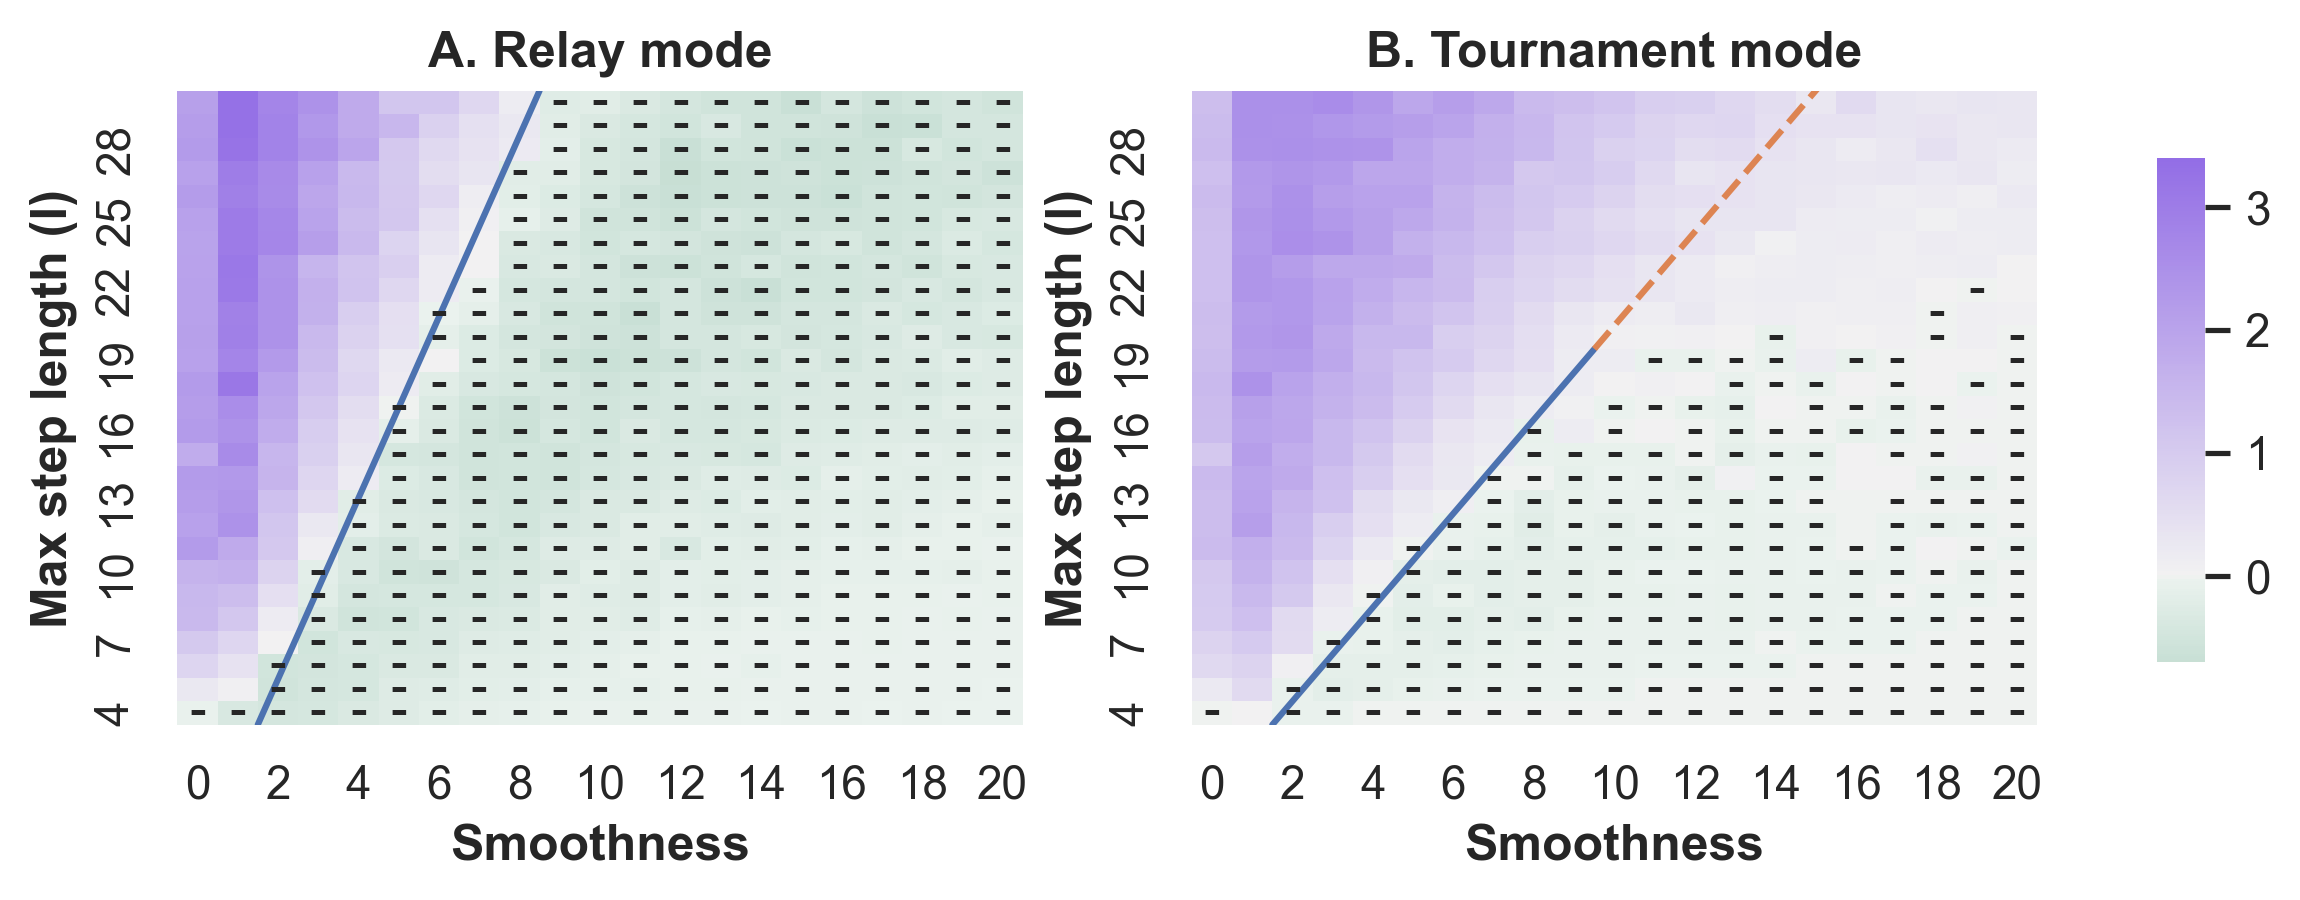
\includegraphics[width=\linewidth]{Fig69.png}
   \caption{Performance of random teams versus high-ability teams over 100 random landscapes for different levels of smoothness and maximum step lengths (where bigger maximum step length creates a larger heuristics pool). Positive values indicate that 'diversity trumps ability', all combinations where the average is negative are marked with the '-' symbol.}
   \label{fig:Grim69}
 \end{figure}
 
 The results closely replicate those presented in Figures 6 and 9 in Grim and colleagues.\footnote{The results also confirm the claim by Hong and Page that the strategy chosen made little difference to their results, given that the first columns with a smoothness factor of 0 look very similar across the panels.} Panel A in Figure \ref{fig:Grim69} shows that, as per the original article, "for heuristic pools roughly three times the smoothing factor or greater", random teams outperform the highest-ability teams. Under the tournament dynamic, random teams outperform highest-ability teams more often. They \textit{substantially} outperform high-ability teams when the maximum step length is more than twice the smoothness factor within the range considered by Grim and colleagues. Above that size of the heuristic pool (\textit{l} = 20), they tend to outperform high-ability teams substantially more frequently. This indicates a non-linear relationship, though the range here is insufficient to estimate the functional form. \\
 
 \begin{table}
  \centering
  \caption{Summary of results across 56,700 runs of varying smoothness and step lengths, showing asymmetry in distribution of winning margins}
  \label{tab:win_comp}
\begin{tabular}{lrrrrrr}
  \toprule
  \multicolumn{3}{c}{}& \multicolumn{4}{c|}{Winning margins}\\
  Strategy & \multicolumn{2}{|c|}{Random team performance} & \multicolumn{2}{l|}{Random team} & \multicolumn{2}{l|}{high-ability team}\\
       &  \multicolumn{1}{|l}{Win rate (\%)} &  \multicolumn{1}{l|}{Mean margin} &  Mean &  \multicolumn{1}{l|}{Max} &  Mean &  \multicolumn{1}{l|}{Max} \\
  \midrule
       Relay &          25.9 &            0.14 &         1.50 &        3.32 &       0.34 &      0.69 \\
   Tournament &          60.0 &            0.54 &         0.93 &        2.58 &       0.06 &      0.21 \\
  \bottomrule
  \end{tabular}
\end{table} 
 
 Visually, the figures presented by Grim and colleagues look rather different from those presented here because their scales include a step-change at zero. Thus, they emphasize that highest-ability groups mostly outperform random groups with the relay strategy, and that the victories are more evenly split with the tournament strategy. This is visible here when one compares the '-' characters, indicating negative values, with the fields without annotation. However, such an emphasis obscures the fact that the highest-ability teams \textit{never} show anything close to the advantage that random teams exhibit when they dominate. For instance, under the relay-strategy, random teams only win 25.9\% of the runs, but still rack up an average advantage of 0.14 \%-age points. Table \ref{tab:win_comp} shows this asymmetry in further detail. It is also worth noting that the tournament strategy leads to better solutions. Both random and highest-performing groups achieved better outcomes with that strategy on 100\% of runs, with high-ability groups gaining 2.3 and random groups 2.8 \%-age points on average.
 

 \section{Conclusion}
 
 Overall, this replication confirms the main results presented in the two target papers. Within the parameters of the model proposed by Hong and Page, randomly selected, and thus diverse, groups outperform groups of the highest ability agents when the solution landscape is fully random. As originally shown by Grim and colleagues, when randomness is reduced, this effect is weakened and eventually reversed. However, it needs to be noted that over the wide range of parameters considered here, the highest-ability teams rarely if ever \textit{substantially} outperformed the random, more diverse, teams. As shown by Grim and colleagues, more independent searches in the form of a tournament strategy and a larger heuristic pool enhance the relative performance of the diverse teams further. \\

 The results indicate various directions for future research. For instance, Hong and Page noted that diversity could be conceptualized both as that of heuristics and that of perspectives, yet research using their model has so far focused on heuristics. Given the poor performance of both types of teams employing hill-climbing heuristics on the smoothed landscapes considered by Grim and colleagues, it might be time to consider different perspectives, for instance in the sense of different starting points. Additionally, further research into the boundary conditions of the "diversity trumps ability" finding is necessary. Such endeavors will hopefully be facilitated by the availability of the model as open code using the mesa framework. 